% !TEX encoding = UTF-8
% !TEX TS-program = pdflatex
% !TEX root = ../tesi.tex

%**************************************************************
\chapter{Progettazione e codifica}
\label{cap:progettazione-codifica}
%**************************************************************

\intro{Breve introduzione al capitolo}\\
Il presente capitolo ha lo scopo di presentare e dimostrare l'architettura per i componenti IW e SP che dovranno funzionare nel contesto dell'estensione del prodotto Monokee.
%**************************************************************
\section{Componente Identity Wallet}
Questa sezione inizia con una generica introduzione all’architettura Xamarin ed infine conclude presentando una prima ipotesi di architettura in formato UML 2.0.
\subsection{Tecnologie e strumenti}
\label{sec:tecnologie-strumenti}
Il componente Identity Wallet è sviluppato come applicazione mobile, questo contesto implica differenti tecnologie che comunicano e interagiscono fra loro. Le funzionalità di persistenza vengono offerte tramite tre diverse tecnologie: file system, blockchain, e server Monokee. La logica di business è implementata usando il framework .NET. L’interfaccia, invece, usa il pattern MVVM (Model View View Model).
L’IW utilizza una classica architettura a strati (N-tier architecture). Trattandosi di un sistema mobile multi piattaforma, questa architettura è stata calata nel contesto e, quindi, si è deciso di basarla sul concetto di Portable Class Libraries (PCL) presentato da Xamarin. 

\subsubsection{Portable Class Libraries PCL}
\gls{pclg}\glsfirstoccur è un approccio alla condivisione del codice tra le diverse edizioni dell’app destinate a diversi sistemi operativi mobili sviluppato da Xamarin. Segue un diagramma esplicativo di come si sviluppa una tipica architettura PCL. Il diagramma in figura \ref{fig:ark-pcl} è tratto da \url{www.xamarin.com}.

\begin{figure}[!h]
    
    \centering
    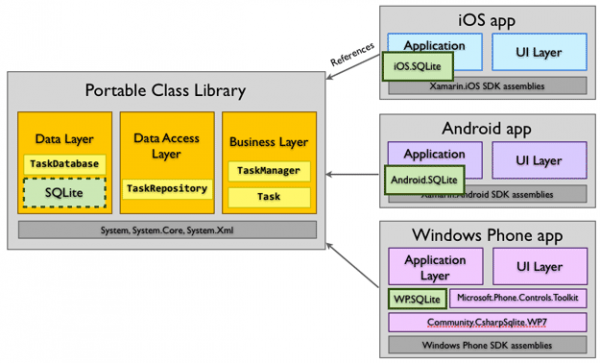
\includegraphics[width=0.9\columnwidth]{ark-pcl.png} 
    \caption{Architettura PCL}
    \label{fig:ark-pcl} 
\end{figure}

Ogni \emph{“Platform-Specific Application Project”} (iOS app, Android app, Windows Phone app) referenzia la \gls{pclg}. Quindi esistono essenzialmente due parti: quelle specifiche per la piattaforma e quelle condivise. Obiettivo del progetto è quello di rendere meno corposa possibile le parti specifiche. Sarà poi possibile impiegare caratteristiche di una determinata piattaforma attraverso l’utilizzo del design pattern \emph{Dependency Injection} (DI).
Applicare i principi della DI significa definire nel codice condiviso interfacce (classi astratte) che vengono implementate (estese) in ogni piattaforma tramite sottoclassi (\emph{Strategy Pattern}). A questo punto, sarà possibile integrare queste specifiche implementazioni all’interno della PCL. Xamarin per questo scopo offre la classe \emph{DependencyService}.


\subsection{Overview}
Come già detto l’applicativo è strutturato come una N-tier application consistente dei seguenti layer:
\begin{itemize}
    \item layer presentazione;
    \item logica di business;
    \item layer di accesso ai dati. 
\end{itemize}
    
Quando si sviluppa un’applicazione è importante scegliere se sviluppare un \emph{thin Web-based client} o \emph{un rich client}. Ovviamente, considerando il nostro contesto ricadiamo nel primo caso, infatti quasi tutta la logica e la persistenza ricadano sul componente ITF. In figura \ref{fig:ark-iw} un'immagine esplicativa dell'architettura ideata.
\begin{figure}[htbp]
    
    \centering
    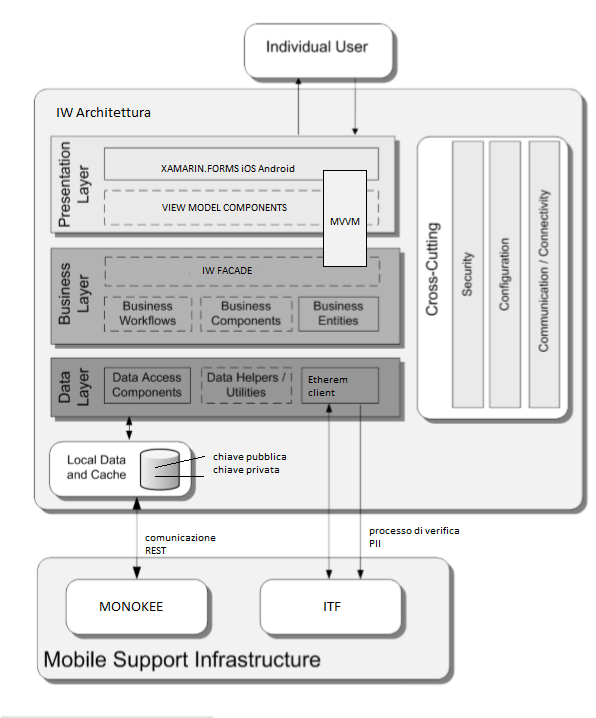
\includegraphics[width=0.9\columnwidth]{ark-iw.png} 
    \caption{Architettura PCWL}
    \label{fig:ark-iw} 
\end{figure}
Come si può notare il principale pattern utilizzato per gestire l’interazione con l’utente è il Model View ViewModel (MVVM). Tutte le elaborazioni vengono effettuate dallo strato di business, mentre per la persistenza ci si affida principalmente o alla risorsa Monokee tramite comunicazione REST, o all’ITF tramite l’utilizzo di un client Ethereum. Tutto verrà sviluppato utilizzando il framework .NET.
%**************************************************************
\subsection{Ciclo di vita del software}
\label{sec:ciclo-vita-software}

%**************************************************************
\subsection{Progettazione}
\label{sec:progettazione}
In figura \ref{fig:ark-mod-iw} viene presentato il diagramma di massima dell’architettura dell’IW. Il diagramma è stata redatto seguendo lo standard \emph{UML 2.0}. Subito a seguire viene descritta ogni classe.
\begin{figure}[htbp]
    
    \centering
    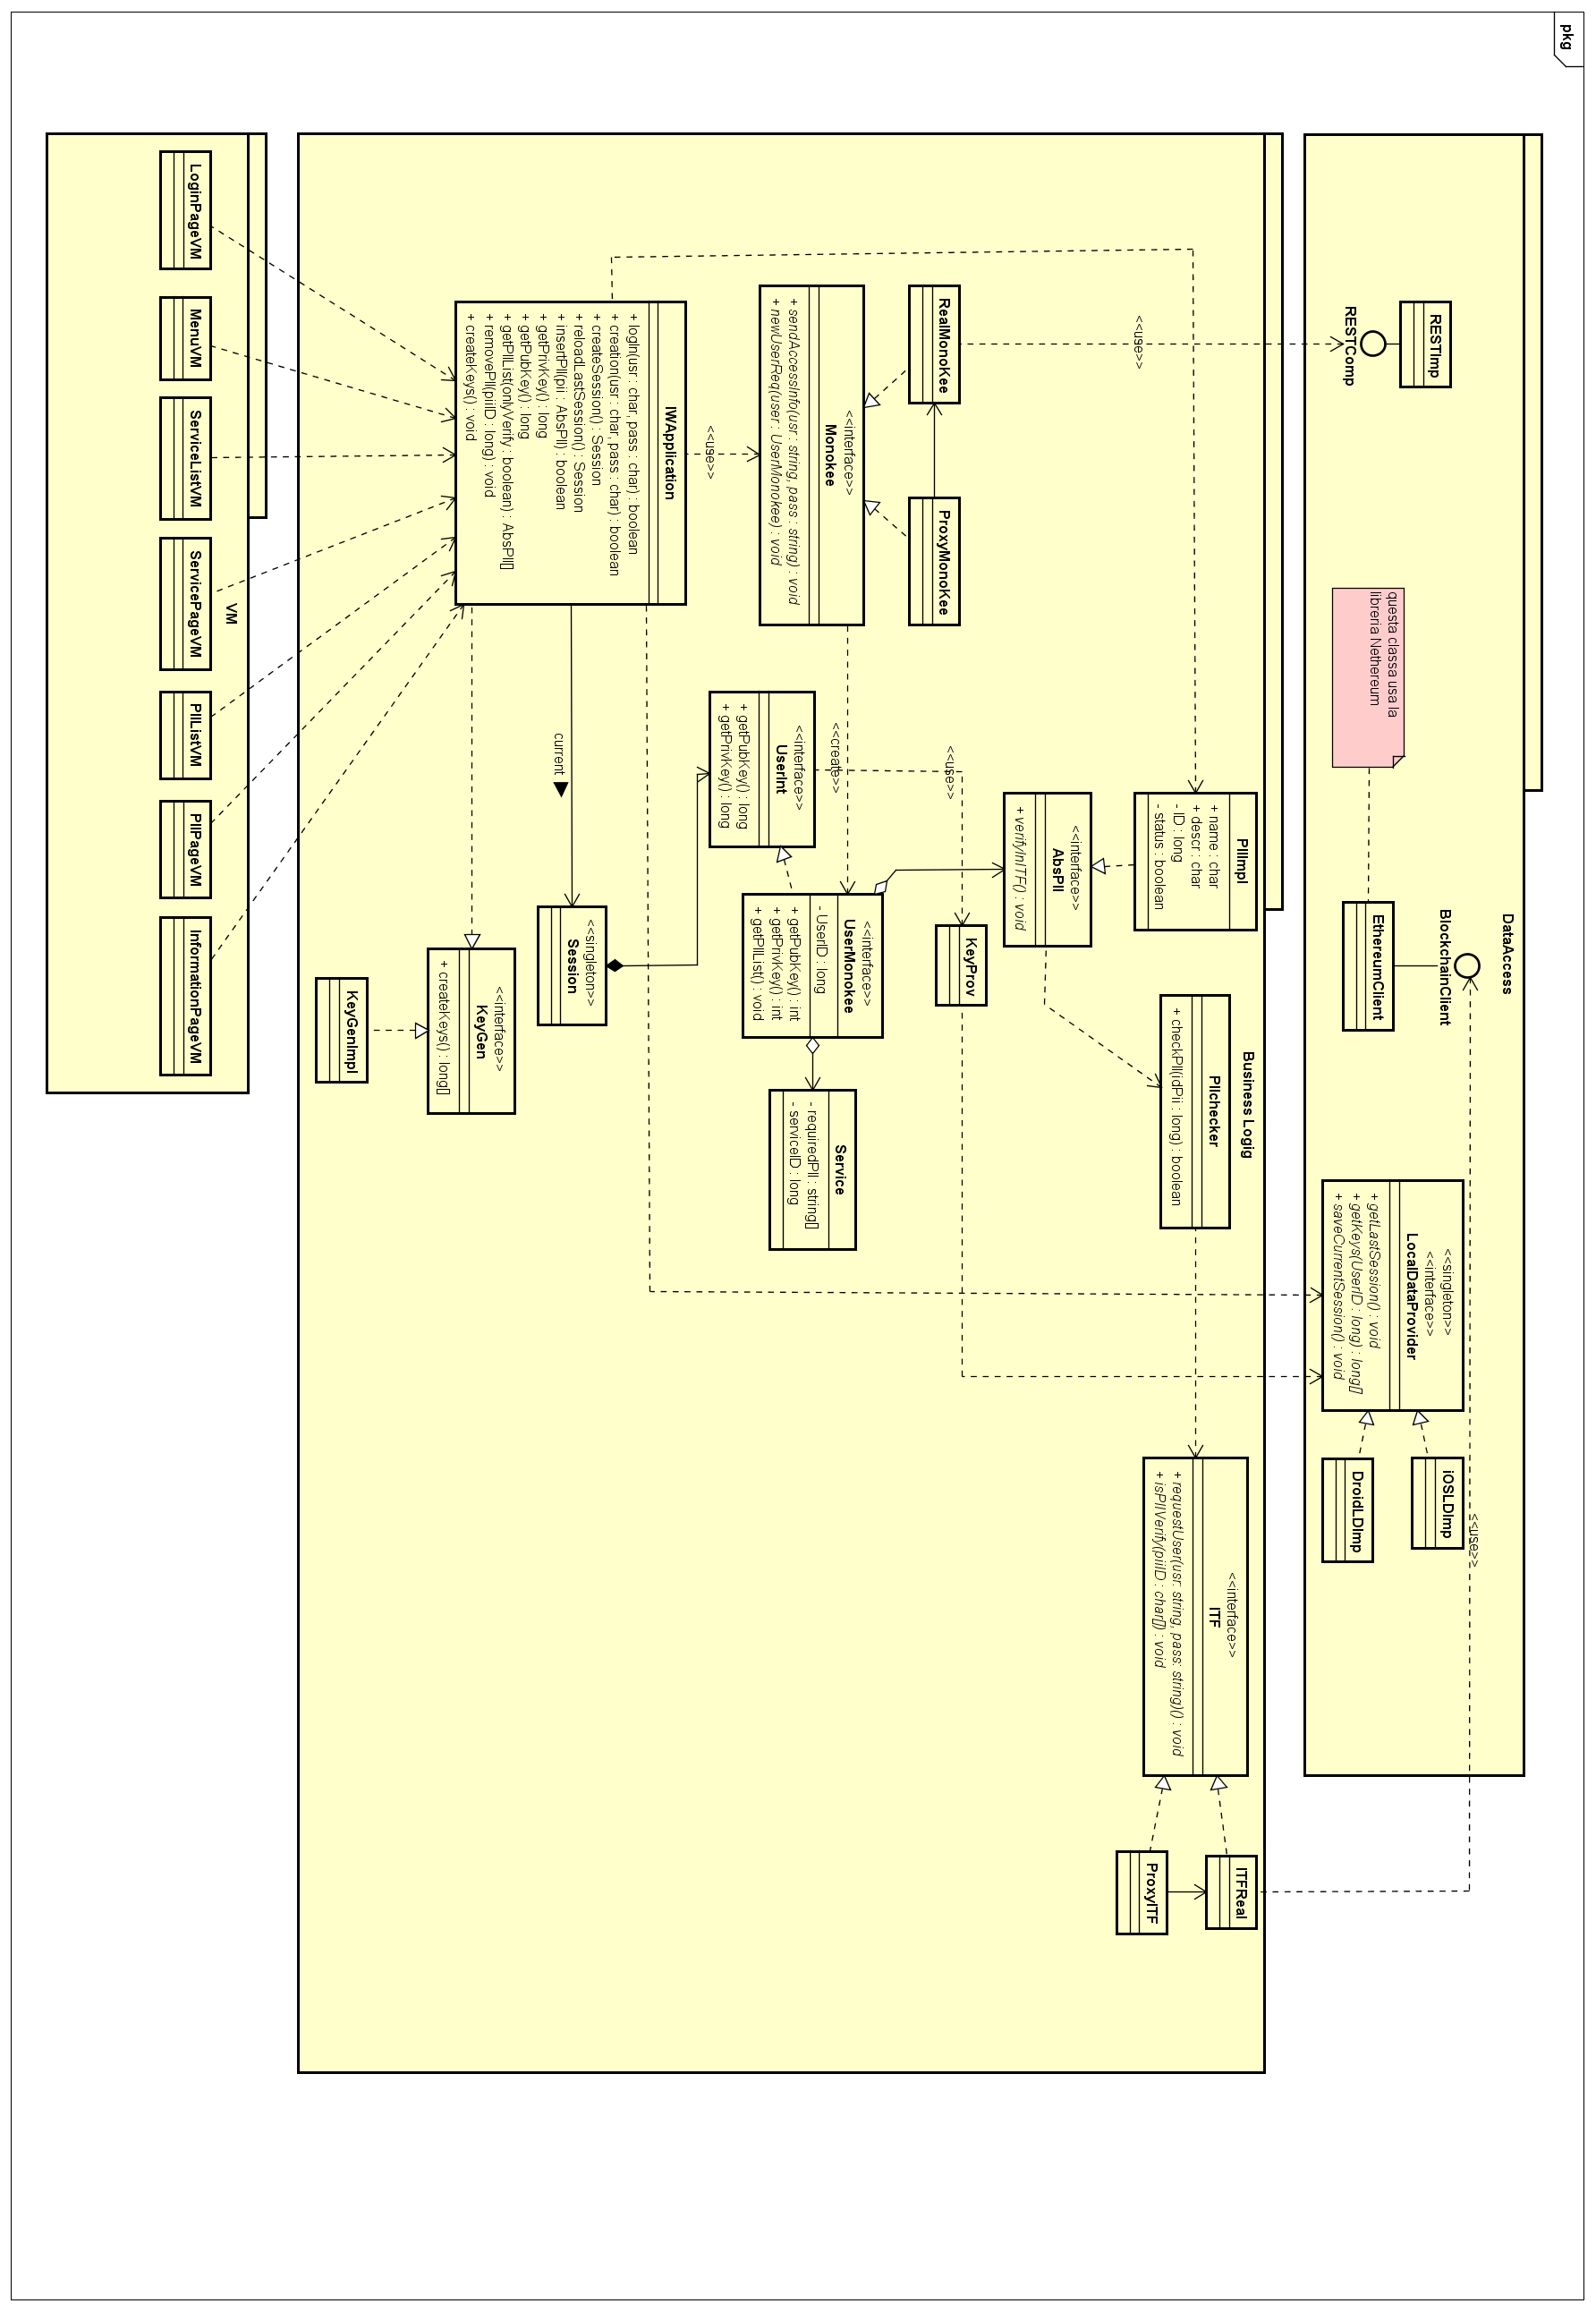
\includegraphics[width=0.9\columnwidth]{ModelArkIW.png} 
    \caption{Architettura IW}
    \label{fig:ark-mod-iw} 
\end{figure}

\paragraph{BusinessLogic} %**************************
\begin{namespacedesc}
    \classdesc{IWApplication}{questa classe ha il compito di fornire una facade per i vari ViewModel. Tutte le azioni possibile tramite l’interfaccia sono quindi implementate da questa classe.}
    \classdesc{Monokee}{ si tratta di un’interfaccia con il compito di fornire un’astrazione del servizio Monokee. Questa interfaccia con RealMonokee e ProxyMonokee rappresenta un’applicazione del pattern Proxy.}
    \classdesc{RealMonokee}{è una classe che rappresenta il reale oggetto Monokee, questa classe poi dialoga con RESTComp per ottenere i dati. Questa classe con RealMonokee e ProxyMonokee rappresenta un’applicazione del pattern Proxy.}
    \classdesc{ProxyMonokee}{è una classe che rappresenta un proxy dell’oggetto Monokee, questa classe applica una politica di acquisizione pigra. Questa classe con RealMonokee e ProxyMonokee rappresenta un’applicazione del pattern Proxy.}
    \classdesc{KeyGen}{è un’interfaccia che ha lo scopo di definire una strategia di generazione chiavi, fa parte di un’applicazione dello Strategy Pattern. È stata pensata in un’ottica in cui ci possono essere vari modi per generare una chiave a seconda del sistema operativo usato.}
    \classdesc{KeyGenImpl}{questa classe rappresenta una possibile implementazione dell’interfaccia KeyGen. Fa parte di un’applicazione dello Strategy pattern.}
    \classdesc{Session}{è una classe con lo scopo di immagazzinare tutti i dati di una sessione attiva, questa può essere generata dal file system o creata da zero. Deve essere presente in istanza singola e contiene le informazioni utente.}
    \classdesc{UserInt}{questa interfaccia rappresenta un qualsiasi utente dell’applicazione. È implementata solamente da UserMonokee. Questo oggetto viene creato dall’interfaccia Monokee.}
    \classdesc{UserMonokee}{è una classe che rappresenta un utente proveniente dal server Monokee. Implementa l’interfaccia Monokee. Un utente di questo tipo possiede un aggregato di servizi, potenzialmente contiene le chiavi e possiede una lista di PII.}
    \classdesc{Service}{è una classe che rappresenta un servizio di cui l’utente ha diritto, possiede un ID e fornisce una lista di PII che dovranno essere presentati al fine di eseguire l’accesso.}
    \classdesc{KeyProv}{è una classe che ha il compito di occuparsi della generazione delle chiavi private e pubbliche. Questa classe viene usata da UserInt e a sua volta usa LocalDataProvider.}
    \classdesc{LocalDataProvider}{è un’interfaccia che ha il compito di fornire in singolo punto dove ottenere informazione dal file system locale. Questa classe poi deve venire implementata in base al sistema operativo su cui girerà. }
    \classdesc{iOSLDImp}{ rappresenta l’implementazione per iOS di LocalDataProvider.}
    \classdesc{DroidLDImp}{rappresenta l’implementazione Android di LocalDataProvider.}
    \classdesc{AbsPII}{è un’interfaccia che rappresenta una generica PII, questa per ora ha una sola possibile implementazione, ma un’interfaccia di questo tipo renderà più semplice l’implementazione di future PII.}
    \classdesc{PIIImpl}{è una classe che rappresenta l’attuale ed unica PII. Consiste di un nome, un identificativo e una descrizione. Una PII può essere verificata o meno tramite l’uso di PIIChecker. }
    \classdesc{ITF}{si tratta di un’interfaccia con il compito di fornire un’astrazione del componente Identity Trust Fabric. Questa interfaccia con ITFReal e ProxyITF rappresenta un’applicazione del pattern Proxy.}
    \classdesc{RealITF}{è una classe che rappresenta il reale oggetto ITF, questa classe poi dialoga con il BlockchainClient per ottenere i dati. Questa classe con RealITF e ProxyITF rappresenta un’applicazione del pattern Proxy.}
    \classdesc{ProxyITF}{è una classe che rappresenta un proxy dell’oggetto Monokee, questa classe applica una politica di acquisizione pigra. Questa classe con RealITF e ProxyITF rappresenta un’applicazione del pattern Proxy.}
    \classdesc{PIIChecher}{è una classe che ha il compito di verificare tramite ITF la veridicità di una PII.}
\end{namespacedesc}

\paragraph{DataAccess} %**************************
\begin{namespacedesc}
    \classdesc{RestComp}{è un’interfaccia che ha il compito di rappresentare una generica strategia di comunicazione REST. Questa viene utilizzata da RealMonokee per ottenere i dati relativi all’utente.}
    \classdesc{RestImpl}{è una possibile implementazione della strategia di comunicazione REST. Implementa l’interfaccia RestComp.}
    \classdesc{BlockchainClient}{è un’interfaccia che ha il compito di rappresentare una generica strategia di comunicazione con la rete blockchain. Questa astrazione permette di slegare dall’architettura dipendenze con le varie implementazioni di blockchain e anche di client.}
    \classdesc{EthereumClient}{è una possibile implementazione di BlockchainClient che utilizza la rete Ethereum. Questa classe poi userà la libreria Nethereum.}
\end{namespacedesc}



\paragraph{PresentationLayer} %**************************
\begin{namespacedesc}
    \classdesc{LoginPageVM}{questa classe ha lo scopo di gestire la pagina di log in e quindi avere lo stato e le operazioni necessarie.}
    \classdesc{MenuVM}{questa classe ha lo scopo di gestire il menu dell’applicazione e quindi avere lo stato e le operazioni necessarie.}
    \classdesc{ServiceListVM}{questa classe ha lo scopo di gestire la pagina che presenta la lista dei service a cui può accedere l’utente e quindi avere lo stato e le operazioni necessarie.}
    \classdesc{ServicePage}{questa classe ha lo scopo di gestire la pagina con le informazioni relative ad un singolo servizio e quindi avere lo stato e le operazioni necessarie.}
    \classdesc{PIIListVM}{questa classe ha lo scopo di gestire la pagina che presenta la lista delle PII che possiede l’utente e quindi avere lo stato e le operazioni necessarie.}
    \classdesc{PIIPageVM}{questa classe ha lo scopo di gestire la pagina che visualizza le informazioni relative ad una specifica PII e quindi avere lo stato e le operazioni necessarie.}
    \classdesc{InformationPageVM}{questa classe ha lo scopo di gestire la pagina che fornisce le informazioni sull’applicazione, sul servizio Monokee e le istruzioni per l’uso.}
\end{namespacedesc}
%**************************************************************
\subsection{Design Pattern utilizzati}
Al fine di garantire elevate doti di qualità e manutenibilità dell’architettura sono stati usati una serie di design pattern. Di seguito segue una breve descrizione di questi.

\paragraph{Communicator}: incapsula i dettagli interni della comunicazione in un componente separato che poi può essere implementato da classi diverse e quindi canali diversi. Questo è risultato utile per rendere gli altri componenti quanto più indipendenti da come comunicano con l’esterno.

\paragraph{Data Transfer Object (DTO)}: è un oggetto che ha il compito di racchiudere le informazioni utili a diverse componenti. Questo riduce i metodi necessari per la comunicazione e in generale la semplifica.

\paragraph{Entity Translator}: Un oggetto che trasforma un dato in una forma utile per essere usato nella logica di business. Questo pattern è stato usato per interfacciarsi con il client Ethereum e il server Monokee.

\paragraph{Lazy Acquisition Proxy}: Ritarda l’acquisizione delle risorse il più a lungo possibile. Questo pattern è stato ampiamente utilizzato, specie per rendere il più leggero possibile la creazione dei dati dell’utente e della verifica dei dati nell’ITF.

\paragraph{Strategy Pattern}: è un oggetto che permette di separare l’esecuzione di un metodo dalla classe che lo contiene. Usando un’interfaccia per astrarre il metodo è poi possibile crearne molteplici implementazioni. Questo è risultato molto utile nel contesto di un’applicazione multi piattaforma in cui alcune procedure andavano implementate in nativo. Oltre all’appena citato vantaggio questo ha reso possibile separare il metodo dall’implementazione.

\paragraph{Dependency Injection}: è un pattern che permette di delegare il controllo della creazione oggetti ad un oggetto esterno. Questo permette di semplificare la gestione delle dipendenze e nel contesto dello strategy pattern permette di inoculare l’implementazione corretta.

\paragraph{Model-View-Controller}: separa il codice per l’interfaccia grafica in tre componenti separati: Modello (il dato), Vista (l’interfaccia), and Controllore (il responsabile della logica), con particolare attenzione alla vista. Nel progetto viene usata una sua particolare declinazione chiamata MVVM. 

%**************************************************************
\subsection{Codifica}


%COMPONENTE SP ********************************************************************
\newpage
\section{Componente Service Provider}
Questa sezione inizia con una generica introduzione alle architetture Event Driven. Viene poi scelto di utilizzare un approccio Broken topology, la scelta è motivata dalla maggiore indipendenza tra i vari componenti rispetto ad un approccio Mediator topology. Infine si conclude presentando una prima ipotesi di architettura in formato UML 2.0.
\subsection{Tecnologie e strumenti}
\label{sec:tecnologie-strumenti}
Il componente Service Provider è sviluppato come applicazione server, questo implica possibili accessi multipli al servizio da parte di vari Real Service Provider (RSP) che inoltrano le loro richieste di accesso. L’applicativo fa uso di diverse fonti per espletare le proprie funzioni. Più dettagliatamente queste sono: Monokee, RSP e ITF. Da questo primo studio architetturale non sembrerebbe necessario l’uso di una base di dati locale.  Considerato quanto appena detto si è ritenuta particolarmente adatta un’architettura Event Driven basata sull’utilizzo di code. Per la comunicazione con il RSP e con Monokee si è deciso di utilizzare un approccio basato sulle API RESTful. Invece per la comunicazione verso l’ITF si è deciso di utilizzare un client Ethereum.

\subsubsection{Architettura Event Driven}
Questo tipologia di architettura rappresenta uno dei principali esempi di pattern architettura asincrono. Produce applicati altamente scalabili e facilmente adattabili ad ogni carico di utilizza. Se applicata bene fornisce la possibilità di avere eventi con un singolo scopo (\gls{srpg}\glsfirstoccur) e con un basso livello di accoppiamento. Questo è reso possibile dalla gestione asincrona di questi eventi.
Ci sono due possibili approcci a questa architettura:
\begin{itemize}
    \item Mediator topology;
    \item Broker topology.
\end{itemize}
\subsubsection{Mediator topology}
Un evento generalmente possiede una serie di passi ordinati per essere eseguito. In questa approccio ci sono quattro componenti che interagiscono fra loro:
\begin{itemize}
    \item una o più code di eventi;
    \item un mediatore di eventi;
    \item uno o più esecutori di eventi;
    \item dei canali di eventi.
\end{itemize}
    
Gli eventi possono essere di due tipi:
\begin{itemize}
    \item eventi iniziali;
    \item eventi di processamento.
\end{itemize}
    
In figura \ref{fig:eventdriver-med-top} si riporta una generica architettura \emph{Event Driven Mediator Topology}.   
\begin{figure}[htbp]
    \centering
    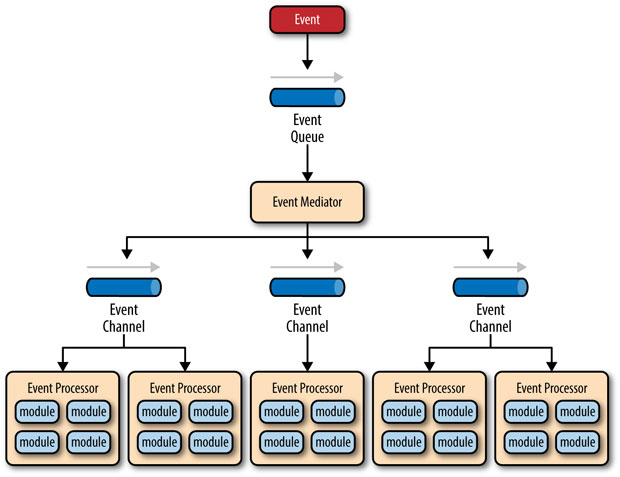
\includegraphics[width=0.9\columnwidth]{med-topology.jpg} 
    \caption{Schema Mediator Topology}
    \label{fig:eventdriver-med-top} 
\end{figure}

\paragraph{Mediatore di eventi}
Il mediatore (l’Event Mediator) ha il compito di orchestrare i passi necessari per rispondere ad un evento iniziale; per ogni passo invia uno specifico evento di processamento ad un canale (Event Channel). Il mediatore non applica nessun tipo di logica, conosce solo i passi necessari per gestire l’evento iniziale e quindi li genera.
\paragraph{Canale di eventi}
Si tratta generalmente di un canale di comunicazione asincrono. Questo può essere di due tipi:
\begin{itemize}
    \item coda di messaggi;
    \item topic di messaggi.
\end{itemize}
\paragraph{Esecutore di eventi}
Contiene la vera logica di business per processo ogni evento. Sono auto contenuti, indipendenti ed scarsamente accoppiati.



\subsubsection{Broker topology}
In questo approccio non è presente un mediatore centrale. Il flusso dei messaggi viene distribuito dai vari esecutori, creando una catena di eventi che generano a loro volta altri eventi. Risulta molto utile nel caso in cui il flusso sia molto semplice. 

In questo approccio ci sono due principali componenti:
\begin{itemize}
    \item un broker che contiene tutti i canali;
    \item vari esecutori di eventi.
\end{itemize}
    
In figura \ref{fig:eventdriven-bro-top} si riporta una generica architettura Event Driven Broker Topology.

\begin{figure}[htbp]
    \centering
    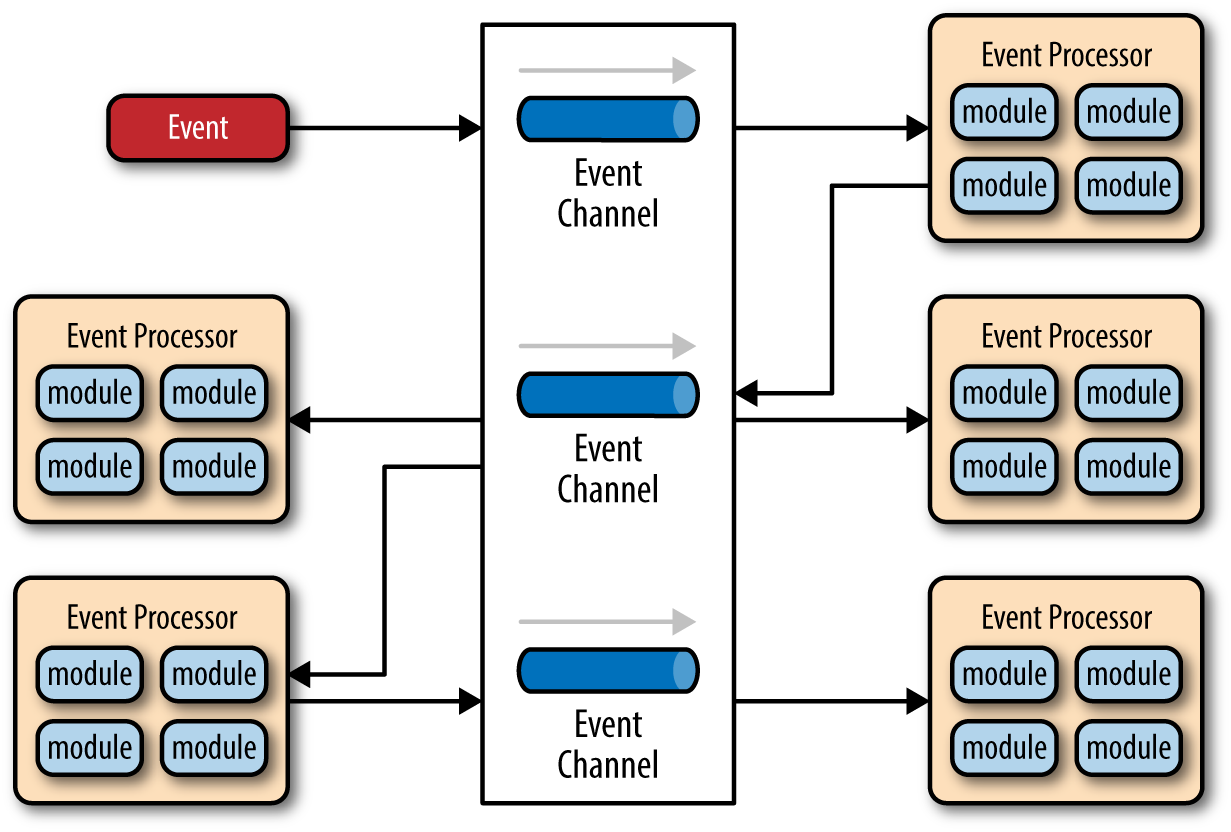
\includegraphics[width=0.9\columnwidth]{brok-top.png} 
    \caption{Schema Broker Topology}
    \label{fig:eventdriven-bro-top} 
\end{figure}

\subsubsection{Considerazioni}
Di seguito si evidenziano alcune vantaggi e svantaggi in maniera analitica \footnote{site:event-driven}:
\paragraph{Agilità generale}
I cambiamenti sono generalmente isolati e possono essere fatti velocemente con piccoli impatti.
\paragraph{Facilità di deploy}
È dovuta all’alto disaccoppiamento degli esecutori. Questa nota vale particolarmente per la tipologia Broker in quanto non presenta il mediatore.
\paragraph{Testabilità}
Richiede strumenti specializzati per generare eventi, questo potrebbe rendere i test di sistema difficoltosi. I test di unità invece sono facilmente implementabili. 
\paragraph{Scalabilità}
La natura indipendente dei componenti rende facile scalare questi in base alle necessità permettendo così un tuning delle risorse molto fine.
\paragraph{Facilità di sviluppo }
È il principale svantaggio di queste architettura.


Uno dei principali svantaggi di questo tipo di architettura è la complessità di implementazione, dovuta al fatto che operazioni sono completamente asincrone e concorrenti. Si è comunque ritenuta questa architettura nella sua variante Broker Topology adatta allo scopo soprattutto per questioni di performance, scalabilità e facilità di deploy.

\subsection{Overview}
Come già detto l’applicazione sarà strutturata con una architettura Event Driven di tipo Broker topology, questo implica che la logica di funzionamento sia incapsulata nei vari passaggi tra le varie code.
Gli esecutori sono i seguenti cinque:
\begin{itemize}
    \item \textbf{Starter}: con il compito di ascoltare gli eventi iniziali dei vari RSP e di ricevere i vari dati ottenuti tramite codici QR;
    \item RetriveInfo: con il compito di ottenere le informazioni necessarie da Monokee;
    \item \textbf{PageResponce}: con il compito di generare e visualizzare le pagine nel broswer dell’utente, sia di fallimento che di comunicazione;
    \item \textbf{PiiDataHandler}: con il compito di verificare i dati nell’ITF e verificare che questi siano sufficienti per effettuare l’accesso;
    \item \textbf{RSPSendingWork}: con il compito di inviare al RSP le informazioni di accesso.
\end{itemize}
    
Gli eventi sono i seguenti:
\begin{itemize}
    \item \textbf{AccessRequest}: generato dallo starter e eseguito dal RetriveInfo;
    \item \textbf{PageResponce}: generato dal RetriveInfo in caso di errore o per mostrare il lettore QR, dal PiiDataHandler in caso di login o in caso di insuccesso della verifica;
    \item \textbf{VerificationWork}: generato dallo Starter per verificare i dati forniti tramite il QR e quelli forniti da RequireInfo siano conformi e verificati; 
    \item \textbf{RSPSendingWork}: generato da PiiDataHandler in caso di verifica positiva.
\end{itemize}
    
 Il diagramma in figura \ref{fig:eventdriven-flusso-code} rappresenta come i vari eventi di lavoro si distribuiscono tra i vari esecutori.

 \begin{figure}[htbp]
    \centering
    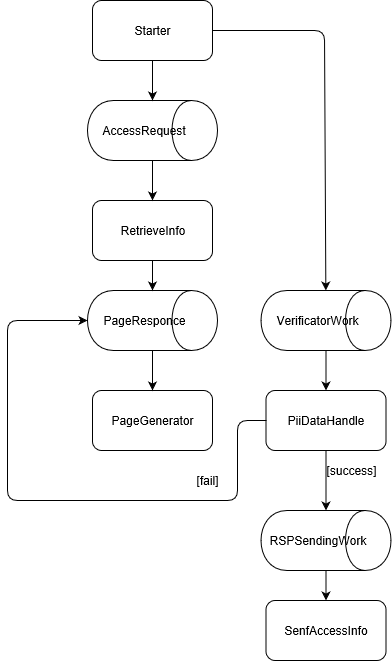
\includegraphics[width=0.9\columnwidth]{flow-eventi-sp.png} 
    \caption{Flusso eventi SP}
    \label{fig:eventdriven-flusso-code} 
\end{figure}
Lo \emph{Starter} quando riceve una richiesta d’accesso da parte del RSP procede a generare il lavoro di \emph{AccessRequest}, una volta ricavati tutti i dati necessari per l’accesso da Monokee, viene affidato al \emph{PageResponce} l’incarico di visualizzare la pagina che richiede l’inserimento del QR. I dati verranno poi inseriti dall’utente e attraverso lo \emph{Starter} verrà creato un lavoro di verifica dei dati inseriti e se questi sono sufficienti ad accedere al servizio, tramite un’ulteriore accesso a Monokee. In caso di esito positivo viene creato un lavoro di invio dati verso il RSP altrimenti verrà visualizzata una pagina di errore.
%**************************************************************
\subsection{Ciclo di vita del software}
\label{sec:ciclo-vita-software}

%**************************************************************
\subsection{Progettazione}
\label{sec:progettazione}
In figura \ref{fig:sp-uml-diag} si presenta un diagramma delle classi che attua la gestione delle code sopra espletata. Il diagramma è stato redatto in formato \emph{UML 2.0}, con leggere modifiche relativo alla rappresentazione delle varie istanze del template \emph{CommandQueue}. Questo è stato fatto al fine di rendere più leggibile e comprensibile il diagramma. Come si può notare sono presenti componenti non presenti nella precedente trattazione. Questi servono per effettuare le comunicazioni con l’ambiente esterno. Si è deciso per questioni di semplicità di non creare code separate.

\begin{figure}[htbp]
    \centering
    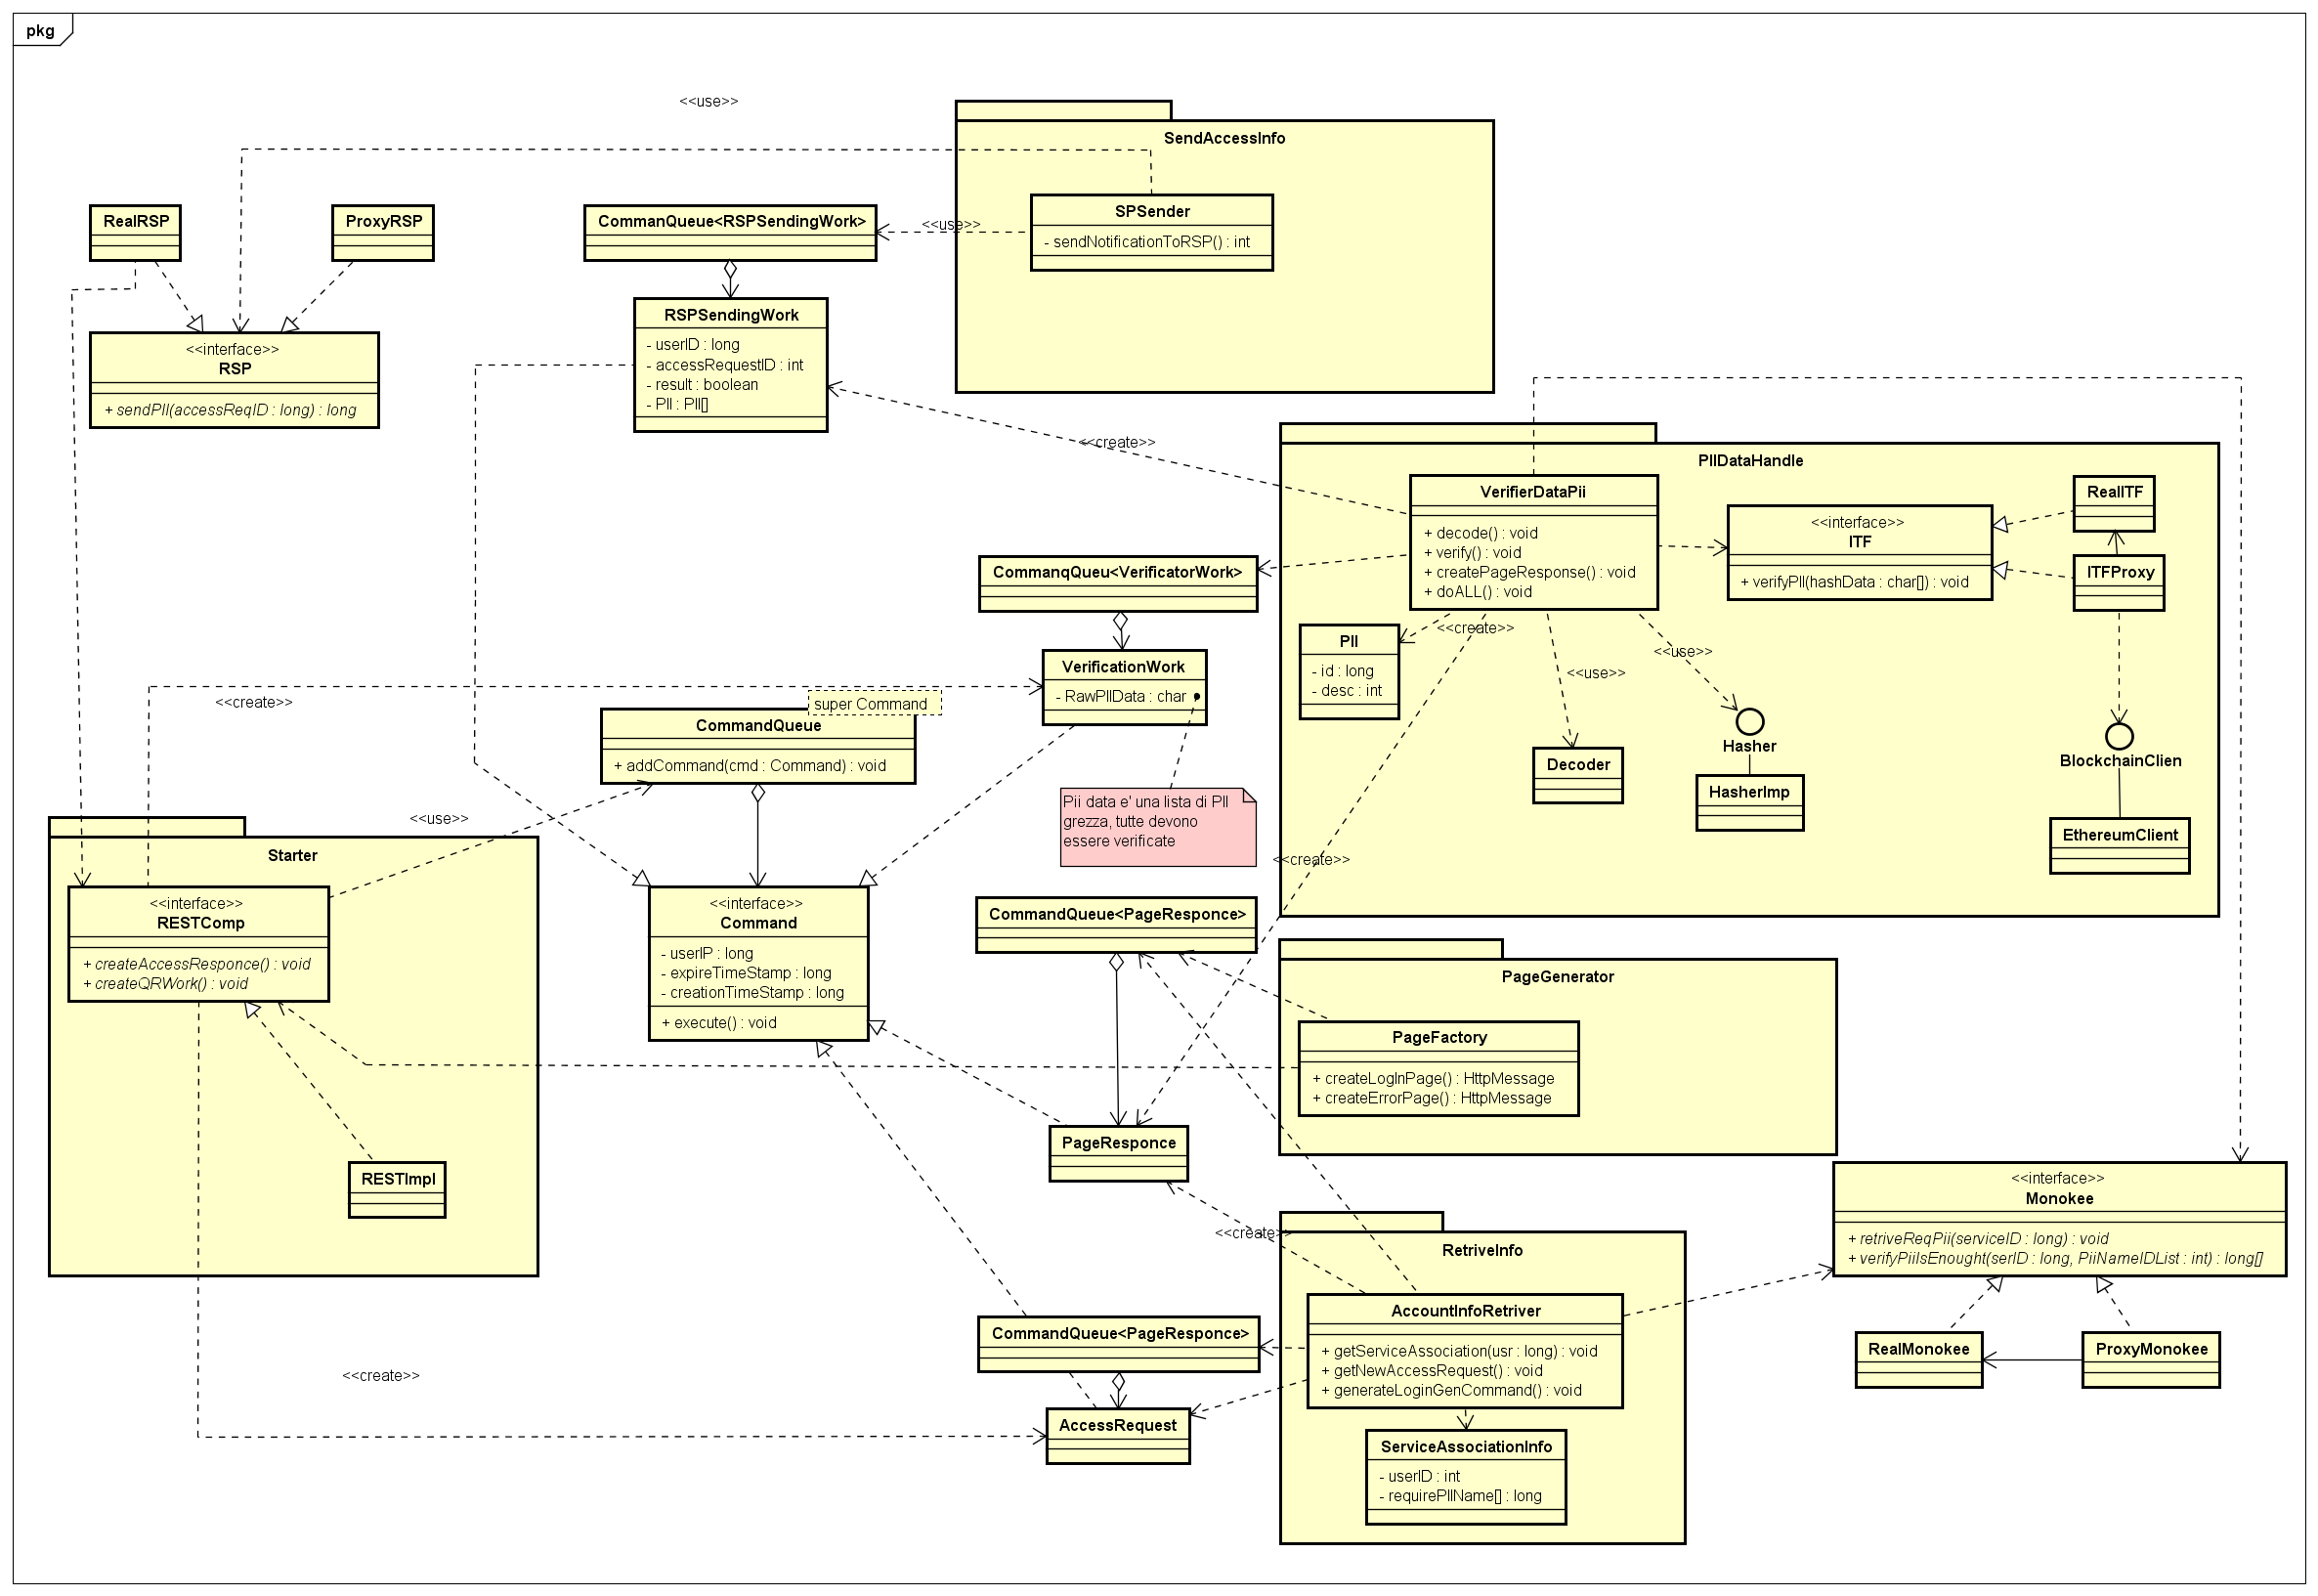
\includegraphics[width=0.9\columnwidth]{SPdiagram.png} 
    \caption{Flusso eventi SP}
    \label{fig:sp-uml-diag} 
\end{figure}

\paragraph{Descrizione elementi} %**************************

\begin{namespacedesc}
    \classdesc{RESTComp}{è un’interfaccia che ha il compito di rappresentare una generica strategia di comunicazione REST. Questa viene utilizzata da RealMonokee per ottenere i dati relativi all’utente.}

    \classdesc{RESTImpl}{è una possibile implementazione della strategia di comunicazione REST. Implementa l’interfaccia RestComp.}
    \classdesc{RSP}{si tratta di un’interfaccia con il compito di fornire un’astrazione del componente real service provider. Questa interfaccia con RSPReal e ProxyRSP rappresenta un’applicazione del pattern Proxy.}
    \classdesc{RealRSP}{è una classe che rappresenta il reale oggetto RSP, questa classe poi dialoga con il RESTComp per ottenere i dati. Questa classe con RealRSP e ProxyRSP rappresenta un’applicazione del pattern Proxy.}
    \classdesc{ProxyRSP}{è una classe che rappresenta un proxy dell’oggetto RSP, questa classe applica una politica di acquisizione remota. Questa classe con RealRSP e ProxyRSP rappresenta un’applicazione del pattern Proxy.}
    \classdesc{Command}{È una classe che rappresenta un generico evento nel contesto dell’architettura event driven. Questa interfaccia viene poi implementata da:
    \begin{itemize}
        \item \textbf{AccessRequest}: generato dallo starter e eseguito dal RetriveInfo, rappresenta il lavoro per gestire la richiesta di accesso;
        \item \textbf{PageResponce}: generato dal RetriveInfo in caso di errore o per mostrare il lettore QR, dal PiiDataHandler in caso di login o in caso di insuccesso della verifica. Rappresenta il lavoro di generazione e sottomissione delle pagine all’utente;
        \item \textbf{VerificationWork}: generato dallo Starter per verificare i dati forniti tramite il QR e quelli forniti da Monokee siano conformi e verificati; 
        \item \textbf{RSPSendingWork}: generato da PiiDataHandler in caso di verifica positiva. Rappresenta il lavoro di sottomissione dati in caso di verifica positiva.
    \end{itemize}
    }
    
    \classdesc{CommandQueue}{Questo template definisce una coda di command. Dispone delle funzionalità per gestire la coda in maniera concorrente.}

    \classdesc{Account Retriver}{È la classe che ha il compito di guidare l’esecuzione di un AccessRequest. }

    \classdesc{ServiceAssociationInfo}{È una classe generata da Monokee che rappresenta un l’associazione tra utente e servizio e il nome dei PII richiesti.}

    \classdesc{Monokee}{si tratta di un’interfaccia con il compito di fornire un’astrazione del servizio Monokee. Questa interfaccia con RealMonokee e ProxyMonokee rappresenta un’applicazione del pattern Proxy.}

    \classdesc{RealMonokee}{è una classe che rappresenta il reale oggetto Monokee, questa classe poi dialoga con RESTComp per ottenere i dati. Questa classe con RealMonokee e ProxyMonokee rappresenta un’applicazione del pattern Proxy.}

    \classdesc{ProxyMonokee}{è una classe che rappresenta un proxy dell’oggetto Monokee, questa classe applica una politica di acquisizione pigra. Questa classe con RealMonokee e ProxyMonokee rappresenta un’applicazione del pattern Proxy}

    \classdesc{PageFactory}{È la classe che si occupa di eseguire l’evento PageResponce e quindi di generare le pagine e inviarle.}

    \classdesc{ITF}{si tratta di un’interfaccia con il compito di fornire un’astrazione del componente ITF. Questa interfaccia con RealITF e ProxyITF rappresenta un’applicazione del pattern Proxy.}

    \classdesc{RealITF}{è una classe che rappresenta il reale oggetto ITF, questa classe poi dialoga con il BlockchainClient per ottenere i dati. Questa classe con RealITF e ProxyITF rappresenta un’applicazione del pattern Proxy.}

    \classdesc{ITFProxy}{è una classe che rappresenta un proxy dell’oggetto ITF, questa classe applica una politica di acquisizione remota. Questa classe con RealITF e ITFProxy rappresenta un’applicazione del pattern Proxy.}

    \classdesc{VerifierDataPii}{È la classe che ha il compito di gestire i VerificationWork, si tratta di un’applicazione di Templete Patter. Ha il compito di verificare le informazioni nell’ITF e di inviare una RSPSendingWork in caso di successo o una PageResponce in caso di fallimento.}

    \classdesc{PII}{È una classe che rappresenta una PII. Contiene l’id, la descrizione di una PII.}

    \classdesc{Decoder}{è una classe che ha il compito di decodificare le informazioni presentate tramite il codice QR e quindi generare una serie di PII.}

    \classdesc{Hasher}{È un’interfaccia che ha il compito di eseguire l’hash di un dato. Rappresenta un’applicazione dello strategy pattern. }

    \classdesc{HasherImpl}{È una classe che implementa un’implementazione della classe Hasher. Esegue l’hash di un dato. Rappresenta con Hasher un’applicazione dello strategy pattern.}

    \classdesc{SPSender}{È la classe che ha il compito di eseguire i RSPSendingWork. Invia tramite il componente RestCompOut le informazioni relative l’accesso al RSP.}

\end{namespacedesc}


%**************************************************************
\subsection{Design Pattern utilizzati}
Al fine di garantire elevate doti di qualità e manutenibilità dell’architettura sono stati usati una serie di design pattern. Di seguito segue una breve descrizione di questi.


\paragraph{Command Pattern} permette di isolare la porzione di codice che effettua un'azione (eventualmente molto complessa) dal codice che ne richiede l'esecuzione; l'azione è incapsulata nell'oggetto Command. 
\paragraph{Remote Proxy} fornisce una rappresentazione locale di un oggetto remoto remote. 
\paragraph{Strategy Pattern} è un oggetto che permette di separare l’esecuzione di un metodo dalla classe che lo contiene. Usando un’interfaccia per astrarre il metodo è poi possibile crearne molteplici implementazioni. Questo è risultato molto utile nel contesto di un’applicazione multi piattaforma in cui alcune procedure andavano implementate in nativo. Oltre all’appena citato vantaggio questo ha reso possibile separare il metodo dall’implementazione. 
\paragraph{Dependency Injection} è un pattern che permette di delegare il controllo della creazione oggetti ad un oggetto esterno. Questo permette di semplificare la gestione delle dipendenze e nel contesto dello strategy pattern permette di inoculare l’implementazione corretta. 
\paragraph{Factory Method} è un pattern che permette di convogliare tutte le funzioni di creazione di vari elementi ad un oggetto unico. 

%**************************************************************
\subsection{Codifica}


